\chapter{Managing User Steering Action Data in a WMS} \label{chap_dchiron}

The second instantiation of WfSteer 
aims at allowing for tracking steering actions with low execution overhead in a large-scale execution in a WMS.
The main difference from the implementation for workflow scripts is that
WMSs are responsible for controlling the parallel execution of the workflow
on the HPC machine. Because of this, an important part of a WMS philosophy
is to provide services that alleviate the burden to the users concerning
parallel execution control issues, such as efficient exploitation of the parallel hardware
and consistent execution. The importance of this for steering action data management
is that the WMS must not only provide services to capture, relate, and store
steering action data, but must also address issues related to keeping the execution
consistent when the user is performing an adaptation and, as any WfSteer implementation,
keep the introduced overhead low.
In this chapter, we present our implementation in d-Chiron.
We discuss design principles (Sec. \ref{d-chiron-design-principles}),
implementation details related to consistency control when the user is adapting the workflow (Sec. \ref{d-chiron-implentation}),
then how the user utilizes the WMS for steering (Sec. \ref{dchiron-utilization}).




\section{Design Principles}
\label{d-chiron-design-principles}

In this section, we present the design principles that drive
the architectural, technological and implementation decisions of WfSteer in a WMS.

\textbf{A Data-centric WMS.} A data-centric WMS follows a similar philosophy
proposed by our dataflow-oriented approach in the sense that the dataflow, rather than the execution flow, is a first-class-citizen (Sec. \ref{subsec_datacentric}).
Chiron \cite{Ogasawara2011algebraic, Dias2015Data-centric}
is the only existing WMS that implements a data-centric approach for workflow management.
As any WMS, it must manage the parallel execution control, however
its main purpose is to provide for powerful online data analytical capabilities to users so they can steer a running workflow.
Chiron always has the most up-to-date data for analysis during an experiment
run, ready for joint analysis of domain, execution, and provenance data because it uses a single, unified workflow database both as its only source of data for
parallel task scheduling data management and to provide for data analysis.
d-Chiron \cite{Souza2015Parallel} is a highly distributed, scalable version of Chiron.
Its main differentiator compared to any other WMS is that it relies on an
 efficient in-memory distributed DBMS to deal with distributed and parallel concurrency control in a large-scale execution. It is a good alternative to keep the execution overhead low while allowing for workflow steering.
 For these reasons, we choose d-Chiron to implement WfSteer concepts.

\textbf{Fast Hybrid Transactional and Analytical Workloads.}
When the user sends an adaptation command,
the WMS needs to react and respond to the user call as soon as possible.
The steering action is delimited by a clause $\alpha$ (Def. \ref{def:steeringaction}), which often delimits the
subset of the dataset in the dataflow that is being steered.
Thus, to implement the steering action in a WMS,
the DBMS managing the workflow database needs to implement efficient indexing and \myabbrev{OLTP}{Online Transactional Processing} querying capabilities
to search for specific subsets in large sets of data.
Additionally, after the users adapt, they can analyze the
consequences of the adaptation. In this case, efficient
analytical queries to perform joins over multiple datasets,
aggregations, sorting, and filters are required to enable users
to perform complex data analyses. Therefore, the DBMS
must allow for both OLTP and OLAP workloads.

\textbf{Consistency Control during a Steering Action.} It is essential
that the data remains consistent within a user steering action.
It is quite complex to guarantee a consistent execution when a user
decides to adapt the workflow, in particular in a large HPC execution and
without stopping the workflow execution.
On the other hand, distributed relational DBMS natively provide atomicity, consistency,
isolation, and durability (ACID) transactions \cite{Ozsu2011Principles}.
The WMS can take advantage of this capability and implement the steering actions in a way to outsource to the DBMS complex transaction control that guarantees consistency.

The in-memory distributed DBMS in d-Chiron is the MySQL Cluster\footnote{https://www.mysql.com/products/cluster}, a relational DBMS that ensures strong-consistent ACID transactions, has a high throughput to deal with multiple concurrent tasks, and it supports both transactional and analytical workloads. Thus, MySQL Cluster is a good choice to follow the presented principles.

\section{Implementation Details}
\label{d-chiron-implentation}

In this section, we discuss the implementation details for user steering action data management in d-Chiron.
The steering action we implemented in d-Chiron is user-steered data reduction.
Since it is a WMS and as such it follows the
philosophy to alleviate the burden to the users concerning
execution control issues, a significant part of the implementation efforts are dedicated to addressing consistency problems when the
user is adapting the workflow (Sec. \ref{consistency-issues}).
Then in Section \ref{further-implementation-details-dchiron} we discuss further implementation details on steering action data management in d-Chiron. Finally, in Section \ref{adaptive-monitoring-implementation} we present our implementation of the adaptive monitoring concepts.


\subsection{Addressing Steering Action Data Consistency Issues}
\label{consistency-issues}

This section describes how a consistent data reduction is implemented in a data-centric WMS.


\subsubsection{Consistency Issues in a User-steered Data Reduction}

The data reduction steering action follows the $Cut$ definition (Def. \ref{def:cut}).
$Cut$ can only operate on input data elements that are waiting
to be processed in the workflow. When a $Cut$ happens, the
dataset $I_{DS}$ that will be reduced is a shared resource between the
WMS engine that is normally processing the workflow in a batch job and
the user who wants to remove a slice, delimited by the criteria $C$, from $I_{DS}$; hence, race
conditions can occur. Suppose, for example, that at a given instant
$t$ in time, the WMS finishes processing a set of data elements
and then needs to get new data elements that were waiting to be
processed. If at the same time $t$, the user decides to cut off some
of those input data elements that were waiting to be processed, the WMS
may go to an inconsistent state because it could try to process elements
that were removed. Or, the user may try to remove a slice that the WMS
already considered to process, thus generating errors. These
inconsistencies are even more likely to occur in a highly concurrent
execution, such as executions on large HPC clusters with thousands of
computing cores, as the ones we use for typical CSE workloads.

To address this problem, we define a \emph{safe} subset of an input
dataset $I_{DS}$ to which the data reduction is applied. We split $I_{DS}$ into
two subsets $G \subset I_{DS}$ and $H \subset I_{DS}$, where $G$ has the input data elements that have already been processed and
$H$ has the elements waiting to be
processed. That is,
$I_{DS} \leftarrow G \cup H |  G \cap H =  \varnothing$.
$H$ is the subset of $I_{DS}$ that is safe to remove a data slice
from. To guarantee this, the WMS must provide lock controls so that
only the subset $H$ will be reduced, as we show next.
Figure \ref{fig:cut_rfa} illustrates the separation of the safe subset and the general view of how a data-centric WMS executes a data reduction using the $Cut$ operator, using an excerpt of the Risers Fatigue Analysis workflow (Sec. \ref{sub_rfa}) as example.

\begin{figure}[H]
    \centering
    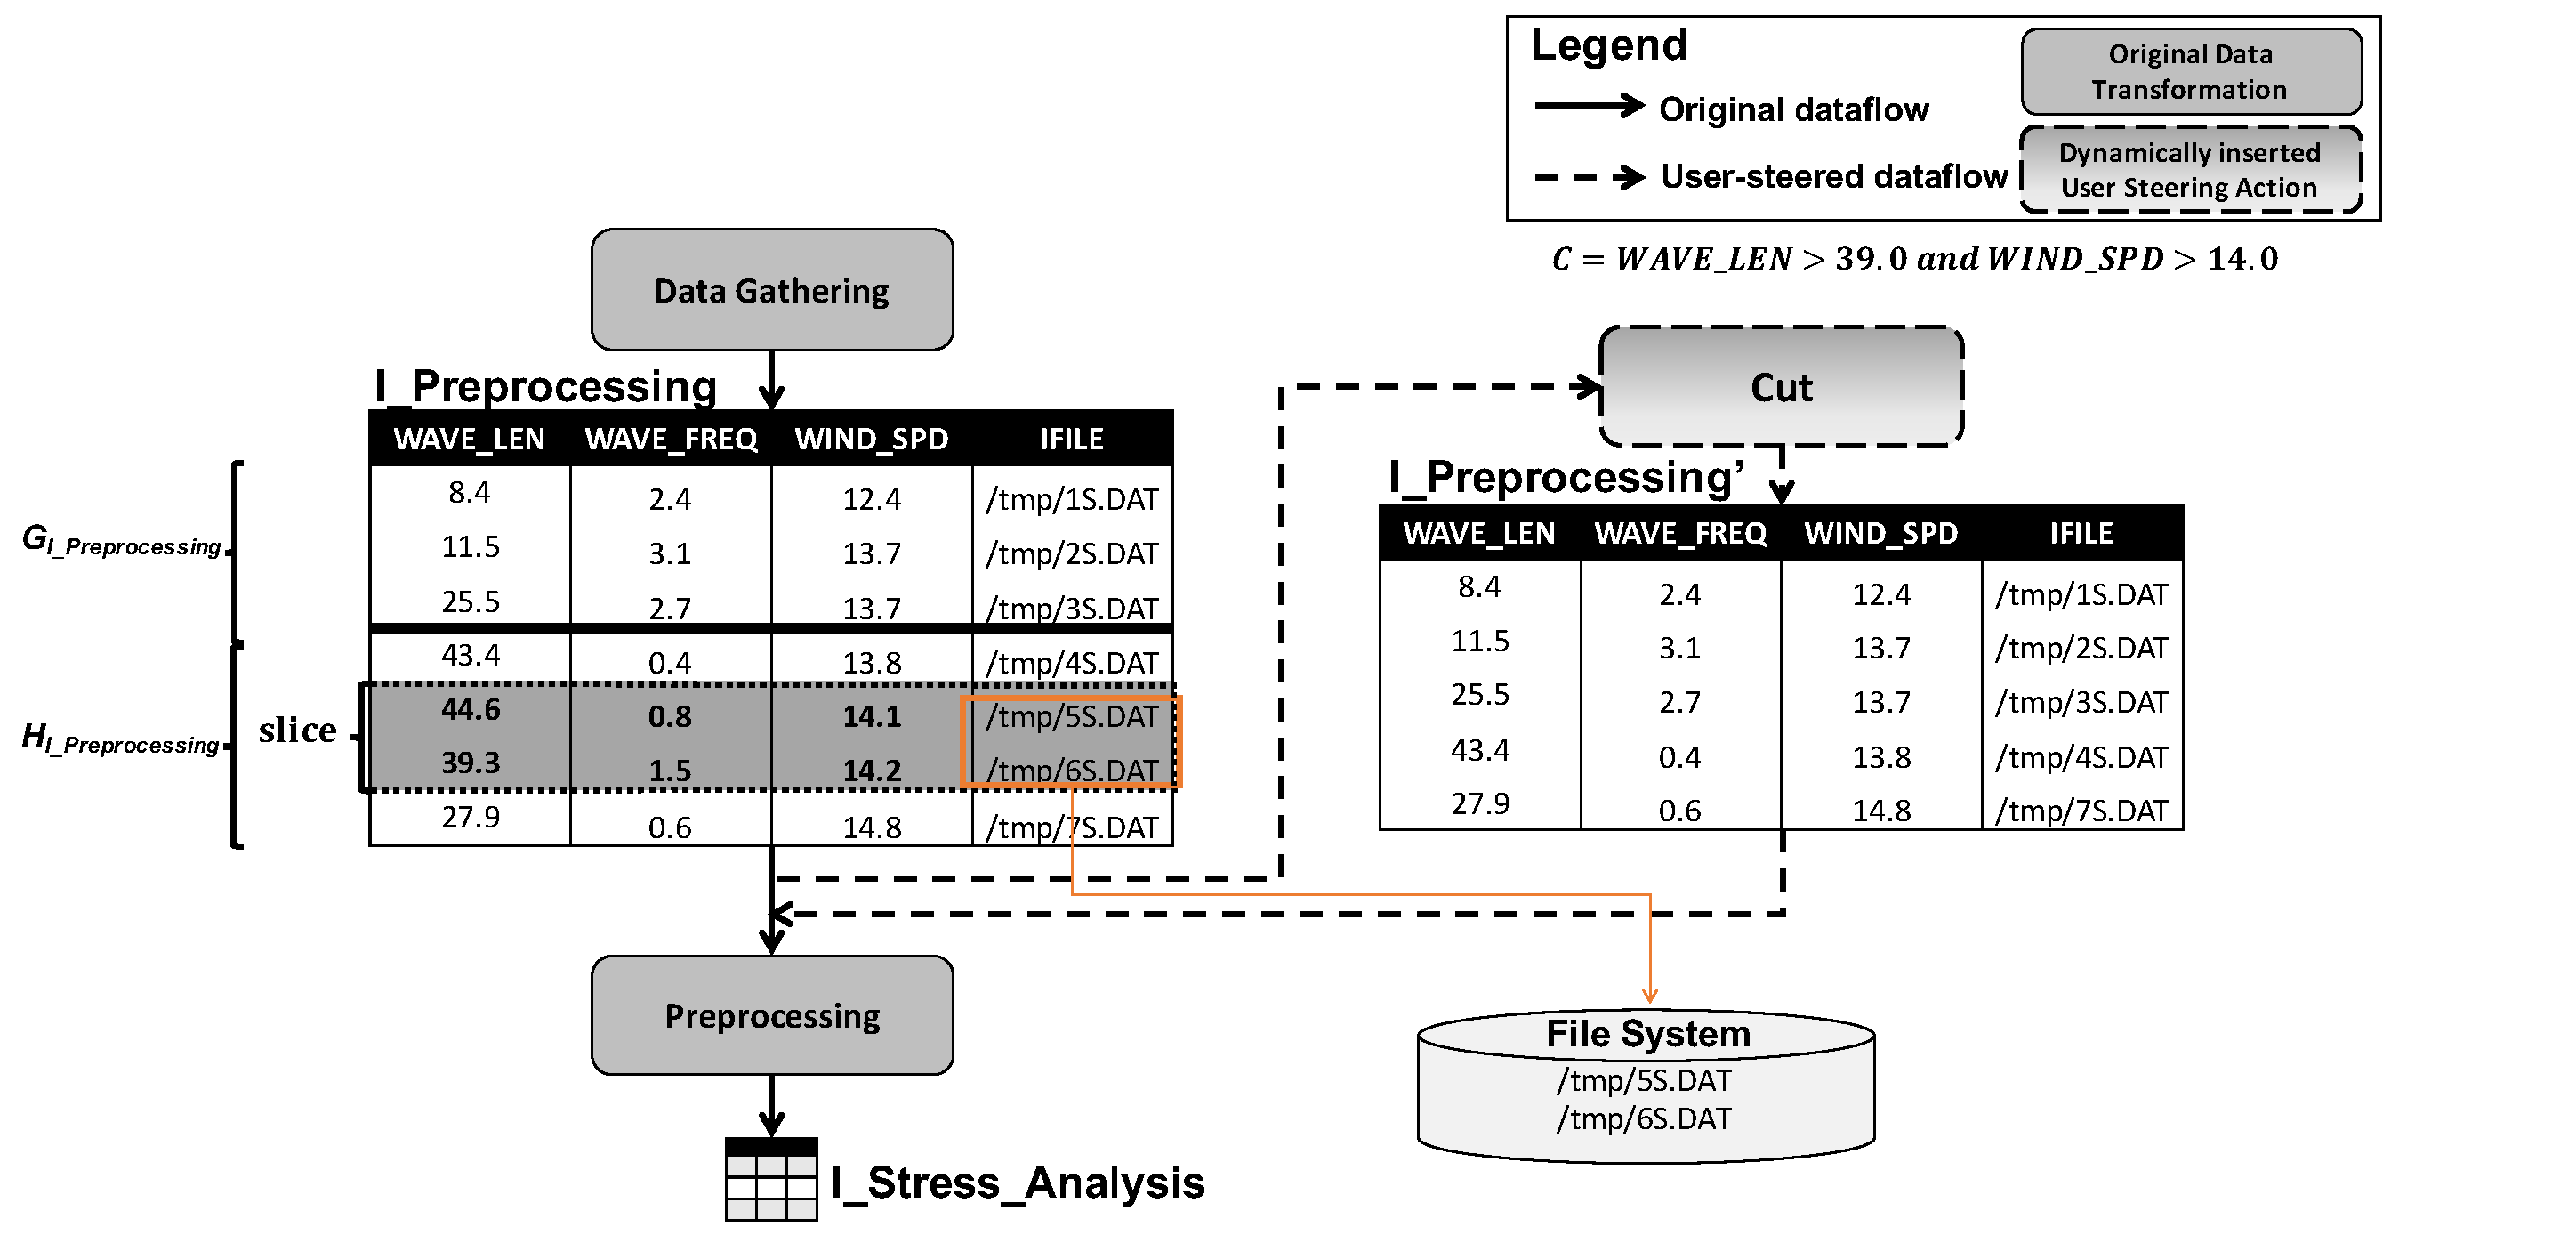
\includegraphics[width=\textwidth,keepaspectratio]{img/rfa_cut_example.pdf}
    \caption{User-steered data reduction using the $Cut$ operator. The input dataset  $I\_Preprocessing$ is split into subsets $G_{I\_Preprocessing}$ and $H_{I\_Preprocessing}$. 
    A slice following the criteria $C = WAVE\_LEN > 39.0 \wedge WIND\_SPD > 14$ is cut off from $I\_Preprocessing$ transforming it into $I\_Preprocessing'$.}
    \label{fig:cut_rfa}
\end{figure}


\subsubsection{Addressing Consistency Issues using a Relational DBMS}

Before diving into the details of consistency issues when effectuating a data reduction at runtime, we explain how the slice delimited by the criteria $C$ is defined in
d-Chiron, using its relational DBMS, so it can later be safely removed
while guarantying consistency after reduction.

Input data elements are
consumed by the many parallel tasks (usually thousands in Many-Task
Computing workflows  \cite{Raicu2008Many-task}) that need to be scheduled by the WMS
engine. To represent the
dataflow-oriented approach (Sec. \ref{subsec_datacentric})
in a relational database schema, the
datasets $DS \in D$ map to input and output specializations of \codefont{Dataset} relations (\ie{} tables), according to the domain modeling of the managed application. The tuples of the \codefont{Dataset} relations map to the data elements $e_i \in DS$. The data transformation executions (\ie{} tasks) are mapped to a \codefont{Task} table,
where each task is related to one or more data elements of a dataset.
% Using the using crow's foot database notation:
% \begin{center}
%     \codefont{Task}
% \includegraphics[width=0.2541in,height=0.11426in]{media/datareduction/image8.png}
%     \codefont{Dataset}
% \end{center}

Thus, for a certain
input dataset $I_{DS} \in D$, the join $I_{DS} \bowtie Task$ returns
a set containing tasks with their input data elements in $I_{DS}$.
Moreover, among other attributes, each task has an important
\(\text{state}\) attribute that determines if a task is READY to be
executed (already knows its input data to start, but is waiting for a
free CPU so it can be scheduled), \codefont{RUNNING}, \codefont{COMPLETED} (already been
successfully executed), \codefont{BLOCKED} (even though there may be free CPUs, the
task does not have the input to start yet), or any other state a task
may assume.
Depending on the data transformation, each task may consume one or more input data elements.
Therefore, we distinguish between
(i) data transformations in which each task consumes one data element (we denote
such tasks as $tasks^{1:1}$, and (ii) data transformations in which each
task consumes more than one data element (we denote them as
$tasks^{1:n}$).

(i) In data transformations with $tasks^{1:1}$, removing input data
element means ``informing'' the WMS not to execute the tasks that would
consume them, hence reducing overall execution time.
To implement the separation of the input dataset $I_{DS}$ into $G$ and $H$, a semi-join relational operation \cite{Ozsu2011Principles}
is used to join input data elements from the input dataset $I_{DS}$
with tasks in \codefont{READY} state to only select the domain data
elements that still need to be processed. Then, after having $H$,
the WMS can obtain the elements in $H$ that follow the criteria
$C$.
Since a set containing both the input data elements together with
the related tasks that will consume them is important for the
implementation of data reduction, we denote this set as $\S^{1:1}$:

$$\S^{1:1} \leftarrow \sigma_C(I_{DS}) \ltimes \sigma_{state = READY}(Task)$$

\noindent where the ratio 1:1 means that the tasks in this set are
$tasks^{1:1}$ and the
criteria $C$ is defined in the $Cut$ operator. Finally, the
WMS will know that tasks in $\S^{1:1}$ should not be processed.

(ii) In data transformations with $tasks^{1:n}$, a data reduction in an
input dataset $I_{DS}$ can only occur if the task that will consume
them is in a \codefont{BLOCKED} state.
The task has not started yet because the
needed input data for it to start is still being generated by a running
task in a previous data transformation. When this running task finishes, it signals
that the \codefont{BLOCKED} task can start. While it is still blocked and the input
data elements are being generated, the user can analyze them and
identify data values that can be removed. In this case, we denote the
set $\S^{1:n}$ similarly to the previous one, but it rather returns the
input data elements in $I_{DS}$ that are being consumed by the tasks in
\codefont{BLOCKED} state:



$$
\S^{1:n} \leftarrow  \sigma_C(I_{DS}) \ltimes \sigma_{state=BLOCKED}(Task)
$$
where the ratio 1:n means that the tasks in this set are
$tasks^{1:n}$. Finally, the WMS will know that tasks in $\S^{1:n}$
should not be processed. This is different for
$tasks^{1:1}$ because they cannot be executed if their input
datasets are removed. 
The WMS will know how to handle the tasks in
sets $\S^{1:1}$ or $\S^{1:n}$. For this, it needs to know beforehand, using prospective provenance, 
whether the data transformation corresponding to the tasks that would consume the elements defined
by the criteria $C$ is expected to consume one element per task or many elements per task.
Such verification is important to guarantee
consistency during reduction.



\subsection{Further Details}
\label{further-implementation-details-dchiron}

\subsubsection{Implementing Steering Action-related Consistency Control in d-Chiron}

To ease slice removal in d-Chiron, we developed a program to be used as a command line-based user interface to steer the workflow in d-Chiron.
Similarly to what we did for DfAdapter, we call this program as \codefont{WfSteerCtl}.
With \codefont{WfSteerCtl}, users can issue command lines to inform the name of
the input dataset $I_{DS}$ and the criteria $C$.
The slice delimited by $C$ is added to
the \codefont{where} clause in the SQL query that will form the
\codefont{select} expressions.
As an implementation decision, instead of
physically removing the input data elements (either in $\S^{1:1}$ or
$\S^{1:n}$) from the workflow database, we move them to a \codefont{Modified\_Elements}
table, maintaining the relationships. Likewise, the tasks in
$\S^{1:1}$, which cannot be executed, are not physically removed, but
they have their state marked as \codefont{REMOVED\_BY\_USER}. By doing so, we
enable these tasks and data elements to be later analyzed with
provenance queries.

To guarantee consistency, we take advantage of d-Chiron's DBMS with ACID
transactions. In a user-steered data reduction, both d-Chiron's engine
and the \codefont{WfSteerCtl} program need to concurrently update shared resources: \codefont{Task}
and \codefont{Dataset} tables in the workflow database. The \codefont{WfSteerCtl} program knows if
it is about to reduce data elements within a slice of the type
$\S^{1:1}$ or type $\S^{1:n}$, since it depends on the dataset being
reduced, which is a parameter to the module. Considering the input
data elements (either in $\S^{1:1}$ or in $\S^{1:n}$), while
d-Chiron's engine gets the input data elements to execute, the \codefont{WfSteerCtl} program needs to concurrently move the cut off input data elements to the
\codefont{Modified\_Elements} table. Considering the tasks in
$\S^{1:1}$,
the \codefont{Task} table is a shared resource because while d-Chiron's engine
updates the runnable tasks (select them, update their status to \codefont{RUNNING},
execute them, and mark them as completed), \codefont{WfSteerCtl} needs to update the
\codefont{Task} table to mark the tasks as removed by the user, so that the engine will
not get them for execution.
These concurrent actions make concurrency
control critical.
Figure \ref{fig:seq_diagram_data_reduction}  illustrates these steps with a sequence
diagram. The \codefont{WfSteerCtl} program acts concurrently with the WMS engine on the
shared resources, which are in red in the figure. The steps 1--3 in \codefont{WfSteerCtl}
are put together in a single DBMS transaction,
\ie{} it is atomic.

\begin{figure}[H]
    \centering
    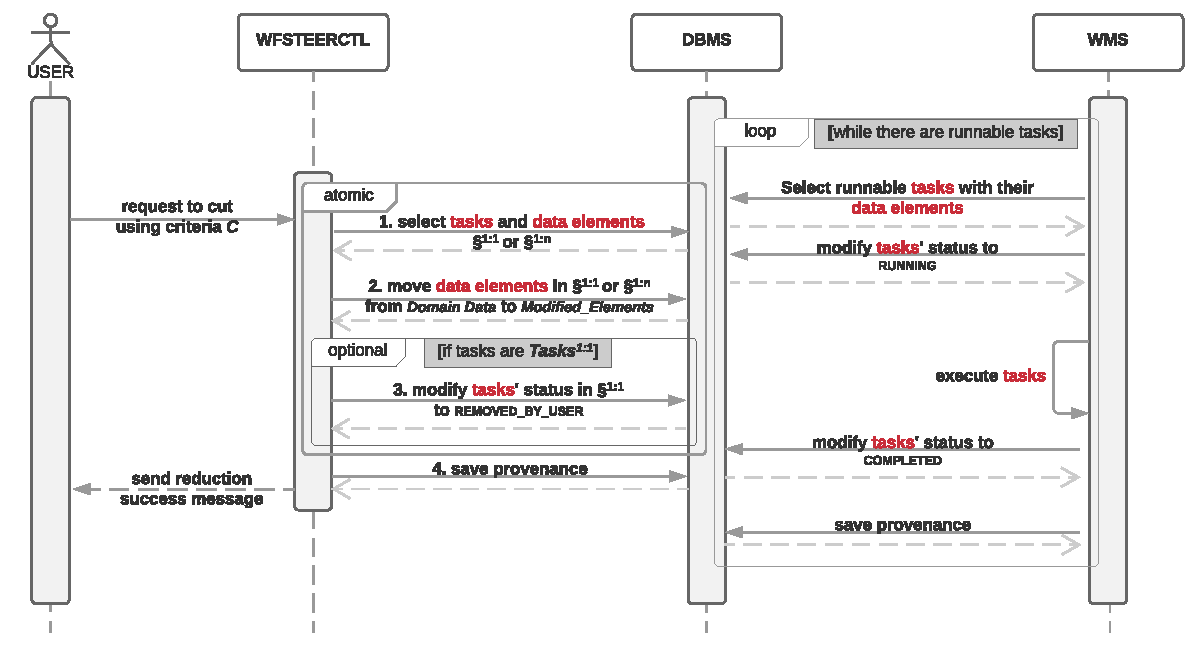
\includegraphics[width=6.06299in,height=3.30315in]{img/dChironSeqDiagram.pdf}
    \caption{Sequence diagram showing what happens in a user-steered data reduction.}
    \label{fig:seq_diagram_data_reduction}
\end{figure}

The workflow database tables are distributed, thus making concurrency control
of the tables' partitions even more complex. In d-Chiron engine,
distributed concurrency control in these tables is outsourced to the
DBMS that guarantees the \myabbrev{ACID}{Atomicity, Consistency, Isolation, Durability} transaction properties \cite{Ozsu2011Principles}.
We developed the
\codefont{WfSteerCtl} program in d-Chiron to also exploit the DBMS in a way that the concurrency
caused by the aforementioned updates is controlled by the DBMS.
Therefore, we implement our approach such that both d-Chiron engine and
the \codefont{WfSteerCtl} rely on the DBMS to outsource those complex distributed
locks and releases of shared resources to guarantee that both execution
and data remain consistent before and after a user-steered reduction.

\subsubsection{Workflow Database Schema}

The data schema that governs the data organization in the workflow database
follows PROV-Wf \cite{Costa2013Capturing}, but d-Chiron has extensions to PROV-Wf to accommodate the steering action data. 
Particularly,
\codefont{User\_Query}, \codefont{Monitoring\_Query},
and \codefont{Monitoring\_Result}. Using PROV nomenclature,
\codefont{User\_Query} is a \codefont{PROV Activity} that stores the slice that represents sets of data elements that will be removed. \codefont{Monitoring\_Query}
is a \codefont{PROV Activity} that contains the monitoring queries submitted
by the user in specific time intervals. The monitoring queries generate
\codefont{PROV Entity} \codefont{Monitoring\_Result}
that stores the query results. These extensions, presented in 2017 \cite{Souza2017Data}, are the first extensions to a PROV data diagram for managing steering action data and are the basis for what we defined later for the PROV-DfA data diagram \cite{Souza2018Provenance} (Sec. \ref{sec_provdfa}).

To
store provenance of removed data elements, we extend the workflow database
schema with the table \codefont{User\_Query} to store the queries that select the
slice of the dataset to be removed.
The description for each \codefont{User\_Query}
column is in Table \ref{tab:dchirontab1}.
The removed data elements are stored in table \codefont{Modified\_Elements}, which is a table that represents a
many-to-many relationship between \codefont{User\_Query} and
\codefont{Dataset}.

\begin{table}[H]
\caption{\codefont{User\_Query} table description.}
\label{tab:dchirontab1}
\begin{tabular}
{
m{.20\textwidth}|
m{.75\textwidth}
}
\Xhline{4\arrayrulewidth}
\rowcolor{TableHeaderColor}
\textbf{Column Name} &                  \textbf{Description}                                     \\
\Xhline{3\arrayrulewidth}
\codefont{query\_id}                      & Auto increment identifier                                                  \\
\Xhline{0.1\arrayrulewidth}
\codefont{slice\_query}                   & Query that selects the slice of the dataset to be removed.    \\
\Xhline{0.1\arrayrulewidth}
\codefont{tasks\_query}                   & Query generated by the WMS to retrieve the ready tasks associated.                          \\
\Xhline{0.1\arrayrulewidth}
\codefont{issued\_time}                   & Timestamp of the user interaction.                                                                            \\
\Xhline{0.1\arrayrulewidth}
\codefont{query\_type}                    & Field that determines how the user interacted. It could be “Removal”, “Addition”, and others. \\
\Xhline{0.1\arrayrulewidth}
\codefont{user\_id}                       & Relationship with the user who issued the interaction query.                                 \\
\Xhline{0.1\arrayrulewidth}
\codefont{wkfid}                         & To maintain relationship with the rest of workflow execution data. \\
\Xhline{4\arrayrulewidth}
\end{tabular}
\end{table}




To store the queries in set $QS$ of our adaptive monitoring approach (Sec. \ref{sec_adaptive_monitoring_concepts}), we create the  \codefont{Monitoring\_Query} table, shown in Table \ref{tab:dchirontab2}.
The main advantage of storing
monitoring results in the workflow database (and adequately linking the
results with the remainder of the data already stored in this database)
whenever a monitoring query result is executed is that users can
query the results immediately after their generation. The workflow database
can also serve as data source for data visualization applications. We
add another table: \codefont{Monitoring\_Query\_Result}, shown in Table \ref{tab:dchirontab3}, to store
monitoring results in the workflow database.

\begin{table}[H]
\caption{\codefont{Monitoring\_Query} table description.}
\label{tab:dchirontab2}
\begin{tabular}
{
m{.25\textwidth}|
m{.73\textwidth}
}
\Xhline{4\arrayrulewidth}
\rowcolor{TableHeaderColor}
\textbf{Column Name} &                  \textbf{Description}                                     \\
\Xhline{3\arrayrulewidth}
\codefont{monitoring\_id}                      & Auto increment identifier.                                                  \\
\Xhline{0.1\arrayrulewidth}
\codefont{interval}                   & Interval time (in seconds) between each monitoring query ($d_i$).    \\
\Xhline{0.1\arrayrulewidth}
\codefont{monitoring\_query}                   & Raw SQL query to be executed.                          \\
\Xhline{0.1\arrayrulewidth}
\codefont{wkfid}                         & Relationship between the monitoring queries and the current execution of the workflow. In d-Chiron's workflow database, there may be data from past executions for a same workflow. \\
\Xhline{4\arrayrulewidth}
\end{tabular}
\end{table}


\begin{table}[H]
\caption{\codefont{Monitoring\_Query\_Result} table description.}
\label{tab:dchirontab3}
\begin{tabular}
{
m{.3\textwidth}|
m{.65\textwidth}
}
\Xhline{4\arrayrulewidth}
\rowcolor{TableHeaderColor}
\textbf{Column Name} &                  \textbf{Description}                                     \\
\Xhline{3\arrayrulewidth}
\codefont{monitoring\_query\_id}                      & Auto increment identifier.                                                  \\
\Xhline{0.1\arrayrulewidth}
\codefont{monitoring\_id}                   & Relationship with the monitoring query that generated this result.    \\
\Xhline{0.1\arrayrulewidth}
\codefont{monitoring\_values}                   & Results of the \codefont{monitoring\_query}.                          \\
\Xhline{0.1\arrayrulewidth}
\codefont{result\_type}                         & Data type of the result values of both queries. Currently, ``Integer", ``Double", ``Array". \\
\Xhline{4\arrayrulewidth}
\end{tabular}
\end{table}



\subsubsection{Adaptive Monitoring Implementation}
\label{adaptive-monitoring-implementation}

Now we provide implementation details for the adaptive monitoring concepts presented in Section \ref{sec_adaptive_monitoring_concepts}.
We implemented a Monitor Manager service that can access the same workflow database used by d-Chiron. A command line starts the Monitor Manager service that runs in the background.
Connection settings
are provided in a configuration file.
Then, the Monitor Manager
keeps querying the \codefont{Monitoring\_Query} table at each $s$ time units to
check if a new monitoring query was added. The default value for $s$
is 30 seconds, as the time interval to check if monitoring queries were
added or removed.
After the service has
started, users can add (or remove) monitoring queries to (or from) the
\codefont{Monitoring\_Query} table.
Currently, users can add monitoring queries
using a command line to inform which SQL query will be executed at each
time interval and the time interval itself.
Whenever the Monitor Manager service
identifies that the user added a new monitoring query, it launches a new
thread. Each thread is responsible for executing each monitoring query $q_i \in QS$, stored in table \codefont{Monitoring\_Query} at each defined time interval $\Delta t_i$. A thread is finished
when a monitoring query is removed or when the workflow stops executing
(in that case, all threads are finished).
Figure \ref{listing:steps_executed_each_interval} shows the steps
executed at each time interval.

\noindent\begin{minipage}[t]{1.0\linewidth}
\begin{lstlisting}[
    caption={Steps executed by each thread within a time interval.},
    label={listing:steps_executed_each_interval},
    mathescape=true
]
Execute the monitoring query $q_i$.
Store query results in the workflow database.
Reload information for $q_i$ from the workflow database for the next time iteration $t + \Delta t_i$. The user could have adapted any of this information.
Wait for $\Delta t_i$ seconds.

\end{lstlisting}
\end{minipage}



To enable these steering capabilities, three of these steps
represent queries to the workflow database, including reads and writes. The
stored results can be further analyzed \emph{a-posteriori} or, more
interestingly, used as input for runtime data visualization tools, since
results are immediately made available after they are generated. In our experiments, Section \ref{sec_exp_rfa_data_reduction_analysis}, we show how users can interact with d-Chiron to add
monitoring queries and use the \codefont{WfSteerCtl} program.


\section{Utilization}
\label{dchiron-utilization}

The ultimate goal of this work is to contribute with user-steered
workflows in HPC. As discussed, \citet{Mattoso2015Dynamic} explain that there are at least
six aspects that need to be considered for this: interactive analysis,
monitoring, user-steered adaptation, notification, interface for interaction,
and computing model.
In this work, we mostly focus on the
first three, considering user-steered adaptation as the core of user
steering and the one we mostly contribute with. As most related
contributions to putting the human in the loop of HPC workflows \cite{Nguyen2015WorkWays:,Mattoso2015Dynamic,Dias2015Data-centric}, we focus on the efforts for designing and implementing concepts behind the backend
enabling technology for user steering in an HPC workflow.
More
specifically, we contribute with allowing users to steer data
reductions in scientific workflows online, focusing on providing a
consistent execution within a data reduction, managing provenance data
of user steering actions, and minimizing performance overheads in the
HPC system. Enabling such features without
jeopardizing performance in an HPC environment is hard.
However, besides engineering the backend enabling technology, the
interface for interaction is another important aspect to be considered.

Designing good interfaces requires usability studies to determine
whether the interfaces are in fact good for the target user profile \ie{} computational scientists in our case.
This would need a
comprehensive user experience test to understand user behavior while
interacting with their workflows, then we would develop interfaces based
on the gathered design insights, and evaluate the usability. For a valid
and comprehensive usability evaluation, we would need to ask multiple
users to use the system and the modules developed, observe how they use,
and interview them. However, the general context that this work is inserted in
very complex. Our target-user profile is quite rare (compared with general
business applications) and the results depend on the domain and the
application in the domain. For example, if we want to measure the time a
user takes to identify that a certain slice will not contribute to the
final results and then remove it, a valid evaluation would require
analyzing multiple users of the same application, in the same domain.
Finding users of a same specific application is so rare that it makes a
comprehensive usability test extremely hard. Also, many other questions
need to be addressed. For instance, ``does the user expertise in the
domain-application interfere in the results? --- perhaps the more
experienced the user is, the faster she will find which slice to remove
and the better she understands the consequences of a reduction''; or
``what if the tests were carried out on a different application for the
same domain?''; or ``what about a different domain?''. Besides, using an HPC cluster requires scheduling. For an usability test, the analyzer needs to observe the user while she is
interacting with the HPC workflow, and thus the analyzer's and the
user's scheduling must match the HPC job scheduling time, for each user.
In other words, a valid and comprehensive usability test would require
observing users of the same application, of different domains, of
different expertise levels, and matching scheduling times with the HPC
cluster. Combining these requirements makes it very hard and out of the
scope of this work, which focuses on enabling backend technology for
steering an HPC workflow.


Therefore, instead of usability tests, in this section, we show how
users can use \codefont{WfSteerCtl} in d-Chiron. Before
developing, we interviewed  a few computational scientists. We found that
they are very used to command line interfaces and they frequently have
to learn new computational tools. They often browse logs in terminals
and follow the execution status of their simulations. To reduce data, they
need to stop their workflow process, modify the input datasets by hand,
and restart execution. For some users, this means resubmitting a job to
an HPC cluster subject to scheduling. This may take  a long time (even
weeks). Therefore, developing a technology that allows them to reduce
data online, based on provenance data analysis through structured
queries (rather than Unix-like shell commands to filter multiple logs in
the file system) is very desirable. Thus,
we developed simple command line interfaces to enable them to steer
monitoring queries and reduce data online. Since developing the best
interface and analyzing its usability is out of the scope, the command
line interfaces are our current best effort to make the technology
usable. As we show in the experiments (Sec. \ref{sec_exp_rfa_data_reduction_analysis}), for validation purposes, a user is
able to use the system, after a d-Chiron specialist trains him and
provided support.

In d-Chiron, computer scientists who are experts in operating d-Chiron
work closely with CSE users, the target-user of this
work. However, computational scientists can operate d-Chiron and
steer the running workflow. Before steering a workflow, the workflow has
to be modeled. The user identifies the input and output data elements of
each of those activities and gives a name to the dataset that contains
those elements (following the dataflow-oriented approach --- Sec. \ref{subsec_datacentric}). When this is done, d-Chiron creates tables corresponding
to those datasets, where each table column is an element produced or
consumed by a data transformation.
If needed, application-specific
extractor scripts are built to collect output data to be stored in the
workflow database \cite{Silva2017Raw}.

The aspects of computational steering workflows tackled in this work are
strongly related to how d-Chiron manages the data and the dataflow. It
is all about the workflow database being populated online by the WMS. The
workflow execution plan depends on the data in this database (hence can
be adapted at runtime) and the workflow database is available for user queries
immediately after the workflow has started to run and data elements in
the domain-dataflow are stored while they are generated. Then, they are
linked to execution and provenance data in the workflow database to enable
queries that integrate all these data.

Therefore, the main way users can interact with a workflow execution in
d-Chiron is through query interfaces, generally provided by the DBMS, to
query the workflow database. It helps to run the queries when the user understands the database schema that logically organizes data in
d-Chiron. Computational scientists or engineers can work with computer scientists
(d-Chiron specialists in this case) so they can build complex analytical SQL
queries to interactively analyze the dataflow. From our experience,
computational scientists do not take much time to learn how to write
simple queries to a relational database and they later learn how to
write complex analytical queries on their own. d-Chiron uses MySQL
Cluster to manage its workflow database. MySQL users are accustomed to using
MySQL Workbench as a visual interface to the DBMS. They can see the
relational database schema, build and run SQL queries, and get their
tabular results in the interface as the workflow runs. Figure \ref{fig:mysql_workbench} shows
how MySQL Workbench can be used to write \refQ{Q5} (described as natural language in Table \ref{tab:queries2}), which integrates domain, provenance
and execution data in a same query. More queries with their natural
language descriptions are on GitHub \cite{d-ChironGitHub} and in the Appendix \ref{sql-codes}.

\begin{figure}
    \centering
   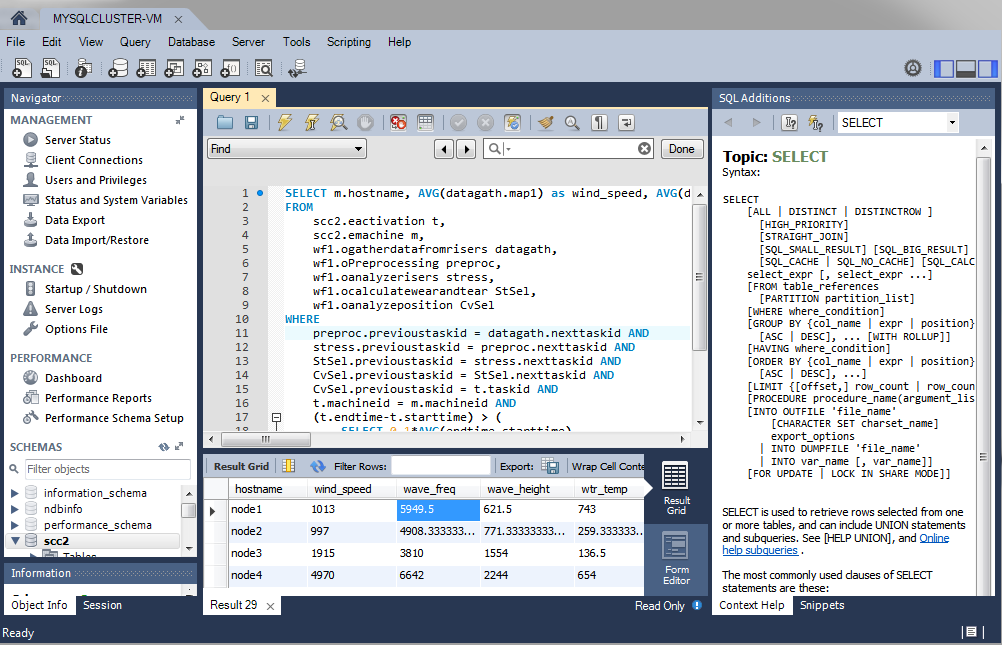
\includegraphics[width=\textwidth,keepaspectratio]{img/mysql_workbench.png}
    \caption{Using MySQL Workbench to query the workflow database at runtime.}
    \label{fig:mysql_workbench}
\end{figure}


However, such user interactivity does not need to use SQL queries only. Some
users prefer graphical user interfaces, so there are many other ways to
interact with a DBMS: graphical interfaces with drag and drop boxes to
help building queries, Natural Language to Database solutions to
translate regular English sentences into SQL queries or dashboards that
plot results from a query. 
In this work, discussing the
usability of interfaces is not the focus. However, we show how
users currently use command line interfaces for the \codefont{WfSteerCtl} program.

For adaptation, a user uses \codefont{WfSteerCtl} program (Figure \ref{listing:dchiron-commandline-steer}) to inform  who is going to
interact (this information
is stored in the workflow database for provenance) and passes a configuration
file that contains information about the workflow, the HPC cluster, and
the DBMS connection settings. After that, a user can run as many
dataflow steering commands as necessary informing the input dataset
$I_{DS}$ in the workflow that will be reduced and the $C$ criteria
to select the slice (operands from $Cut$ Definition \ref{def:cut}).
These steering action data are stored in the workflow database for provenance. The
output messages allow the user to understand what is
happening after a command line is issued. In particular, after a
$Cut$ action, the output message informs the user of the
number of data elements that were removed from the dataset to be
processed. For more complex analyses on the consequences of those
reductions, users can query the workflow database using the tables introduced
in this work to verify, for example, if there were files and their sizes
to quantify the number of bytes that were not processed.
We show these analyses in the experiment section (Sec. \ref{sec_exp_rfa_data_reduction_analysis}).


\noindent\begin{minipage}[t]{1.0\linewidth}

\begin{lstlisting}[
    language=sh,
    caption={\codefont{WfSteerCtl} command line interface for data reduction.},
    label={listing:dchiron-commandline-monitor}
]
$> WfSteerCtl --user="Peter"
    Output: Next workflow interactions will be issued by user Peter.
$> WfSteerCtl --cut --dataset="opreprocessing" --criteria="wind_speed < 12.0 and wave_freq > 2.0"
    Output: 177 data elements were cut off from OPREPROCESSING dataset.
$> WfSteerCtl --cut --dataset="opreprocessing" --criteria="wind_speed < 11.3 and wave_freq > 1.8"
    Output: 55 data elements were cut off from OPREPROCESSING dataset.

\end{lstlisting}
\end{minipage}


For the Monitor Manager service (Figure \ref{listing:dchiron-commandline-monitor}), a user runs a command to start it
 as a background service on any cluster node that has
access to the DBMS, usually the same node from which the WMS execution
was launched. Then, users can add monitoring queries at any time. The
monitoring query results are also properly stored in the workflow database, as
they are generated. Dashboard graphic visualization applications can
query these results to deliver better data visualization for the user.


\noindent\begin{minipage}[t]{1.0\linewidth}
\begin{lstlisting}[
    language=sh,
    caption={\codefont{WfSteerCtl} command line interface for monitoring.},
    label={listing:dchiron-commandline-steer}
]
$> WfSteerCtl --monitor --start
    Output: Ready to accept new monitoring queries.
$> WfSteerCtl --monitor --add --mq="`cat q1.sql`" --label="q1" --interval=30
    Output: Monitoring query q1 will be executed every 30 seconds.
$> WfSteerCtl --monitor --add --mq="`cat q2.sql`" --label="q2" --interval=20
    Output: Monitoring query q2 will be executed every 20 seconds.
$> WfSteerCtl --monitor --update --label="q2" --interval=5
   Output: Monitoring query q2 was updated. It will be executed every 5 seconds.
$> vi q1.sql
$> WfSteerCtl --monitor --update --label="q1" --mq="`cat q1.sql`"
    Output: Monitoring query q1 was updated.

\end{lstlisting}
\end{minipage}




In this example, after the user starts the monitoring service (line 1),
two monitoring queries are added with intervals 30 and 20 seconds,
respectively (lines 3 and 5). The user wrote the queries in text files
(\codefont{q1.sql} and \codefont{q2.sql}), which are loaded in the
\codefont{WfSteerCtl -\/-monitor -\/-add} commands,
using \codefont{cat} Unix command. Those query files are only to facilitate the
command lines and they are not a requirement. A user could write the
query string directly in the command line. After some time, the user decides
to decrease the time interval in the monitoring of query with label
``q2'' by issuing the command at line 7. In line 9, the user decides to modify a
specific query aspect (\eg{} increase the result limit) by
editing the query text file and in line 10 he modifies the monitoring
query. As for the management of steering actions, these user interactions are properly stored in the workflow database for
provenance.

In the next chapter, we present the experimental evaluation of WfSteer.